\begin{figure}[t]
\centering
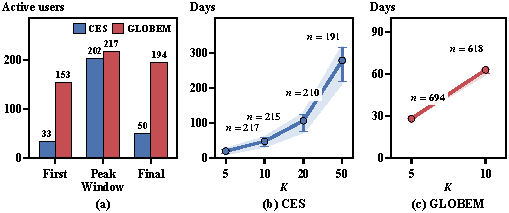
\includegraphics[width=\columnwidth]{figures/fig_streaming_characteristics.pdf}
\caption{Dataset analysis for CES and GLOBEM. (a) Active users in the earliest window (First), the window with the most active users (Peak), and the latest window (Final). (b--c) Median days required to collect the first $K$ feature--label pairs in CES and GLOBEM; shaded areas and error bars show the interquartile range, and $n$ denotes the number of users reaching each $K$.}
\Description{Three-panel dataset analysis. The first panel compares active-user counts across representative temporal windows. The second and third panels show the time required for users to accumulate evidence in CES and GLOBEM.}
\label{fig:dataset-analysis}
\end{figure}
